\chapter{Methodology}

%\section{Overview}

\section{Lightly supervised data selection approach}
\label{lsselection}
Despite of the high development in automatic speech recognition, there exist many challenges. One of the main challenge of speech recognition is to reduce development cost when adapting the speech recognition to other task or creating a new speech recognition for a new language. The biggest development cost is to transcribe the audio data with their exact corresponding transcriptions. To generate a "good" speech recognition, one needs a massive number of training audio and their exact transcriptions. However, transcribing audio is labor intensive and time consuming too. There are unlimited supply of audio data in the internet, television, radio, and other sources. Nonetheless, they usually have a few or even no accurate transcription at all.  Some television broadcasts have corresponding closed captions.  Closed caption means that the transcription is close, but not exactly the same as what the audio says. Even, the closed captions are often badly time-aligned with the audio.

By utilizing these audio data with the corresponding closed captions, we hope to produce a high performance speech recognizer with less supervision. The main idea is to use the automatic speech recognizer to transcribe audio data which will automatically generate transcriptions, which later be used as training data \cite{lightlySupervised}. The steps are as following. Firstly, we train a bootstrap acoustic model trained on a small manually annotated data. Then, recognize the data with closed captions by using the bootstrap model. We compare the decoding result from the bootstrap model with the closed captions and remove the words which do not agree. Finally, we can train a new acoustic model from the filtering.

The idea of using untranscribed audio data has been explored before(Zavaliagkos and Colthurst in 1998 \cite{Zavaliagkos1998UtilizingUT} and Kemp \& Waibel \cite{Kemp_unsupervisedtraining}), which is called as unsupervised acoustic model training. They utilized small amount of audio data without transcription to train acoustic models. The drawback of their experiments is not using massive volume of training data which is essential to train an acoustic model.

Lightly supervised approach was proposed in 2002 by Lamel et al \cite{lightlySupervised}. 
In general, the lightly supervised approach operates as following:
\begin{enumerate}
\item Train an acoustic model on a small amount of manually annotated data. 
\item Recognize(or automatically transcribe) a massive amount of data.
\item Align the automatic transcriptions with the closed captions. Some transcriptions and closed captions might disagree. We can remove or correct these segments.
\item Retrain a new acoustic model using the data which we selected in the previous step. 
\item Reiterate from step 2.
\end{enumerate}
These steps can be iterated several times as long as the error rate is decreasing. This method uses the idea of training acoustic model in less supervised manner because the training dataset(closed captions) is not the real detailed transcription. 

Using closed caption as training data reduces effort in manual transcription.Detailed transcription process usually takes 20-40 times manual effort compare to live closed captioning. Closed caption is usually produced in real time and less costly compare to the detailed transcription. In addition, the manual transcription is possible to have error \cite{Barras2001}. Additionally, some TV broadcasts, such as: CNN headline news, ABC world news tonight, BBC, already have closed captions which can be used as a training dataset. Nevertheless, some problems exist when using the data with closed captions as training dataset. However, training using  the closed captions faces several disadvantages compared to the real transcriptions: indication of non speech event, such as: coughing, speaker turn, acoustic conditions: background noise and music. Furthermore, some sentences might be paraphrased, deleted, and changed in word order. 

In addition to the closed captions, we can use additional data to build a language model. Other kinds of text are available in internet, such as: news, blog, and closed captions from TV broadcast. However, these data might be less related with the audio data. Some additional sources may be not contemporaneous with the data. Thus, it provides less supervision. We can interpolate these data with the closed captions to build a more general language model.

Despite the fact that closed captions are not accurate, it has been proven that closed captions provides enough supervision in building automatic speech recognition systems \cite{lightlySupervised}. Lamel found that an increase in training data improves accuracy even tough it will increase the model size. Additionally, filter closed captions for the next iteration training set in the lightly supervised technique improves the accuracy slightly. The language model built from closed captions also effectively provides enough supervision in building the ASR. Therefore, lightly supervised technique is our main inspiration to do data selection in this internship.

\section{State-of-the-art data selection}
\label{stateoftheart}
Some researches have been conducted to investigate the lightly supervised approach to select data in the speech recognition problem\cite{lightlySupervised,Lecouteux06imperfecttranscript,Chan,Mathias,Stolcke00anefficient}. The state-of-the-art data selection was proposed by  Lanchantin et al from Cambridge university\cite{Lanchantin2016}. Before talking about the state-of-the-art, it is better to discuss some previous related works first.

Lamel et al proposed the lightly supervised approach which harnessed the closed caption as supervision to build a robust speech recognizer\cite{lightlySupervised}. In their experiment, they used a bootstrap acoustic model and biased language model to recognize the audio where the decoding result is compared with the closed caption. Then, the words which do not agree will be removed from training dataset. The new training dataset is utilized to train a  new acoustic model. This filtering(removing not-agree words) is called closed caption filtering.

Chan and Woodland explored another way in filtering bad closed captions\cite{Chan}. They leveraged the confidence measure metric to remove the bad segments. When decoding acoustic inputs, an ASR produces word hypothesis and their corresponding confidence measure. The confidence measure value from each word in  each segment is averaged to produce one confidence value per segment. Finally, they determined a threshold confident value to filter out all potentiallly bad segments, where the confident value is lower than the threshold. Moreover, they also introduced to interpolate two different LMs created from two closed caption datasets and merge them into one single LM. This single LM is used as light supervision when decoding acoustic input together with the acoustic model and the lexicon.

Matias et al applied lightly supervised approach on medical conversation data \cite{Mathias}. There are unlimited supplies of medical speech; however, only informal medical reports are available. The medical reports are not the same as what the physicians said in the audio records. This problem matches perfectly with the lightly supervised approach. They explored frame level filtering in place of word level or segment level filtering. Basically, they forced align and compared the decoding results with the closed captions and mark words which are insertion, deletion, and substitution. All corresponding frames which are associated with those marked words are removed or filtered out from training set to produce a new cleaner training set.

The state-of-the-art data selection was proposed by  Lanchantin et al from Cambridge university\cite{Lanchantin2016}. They used the lightly supervised approach applied on the multi genre broadcast(MGB) challenge. MGB challenge is a challenge to automatically transcribe TV broadcasts. The challenge only provided TV broadcast audio data and their corresponding closed captions. General TV broadcast data are usually recorded in highly diverse environment speech with background music, non speech event, and sound effect. In addition, some closed captions may be different compared to the real transcription due to deletion, insertion, substitution, and paraphrasing. These factors make the challenge interesting as well as complicated. 

Lanchantin et al proposed to tackle the problem inspired from the lightly supervised approach. The lightly supervised approach works as following \cite{Lanchantin2015}.
\begin{enumerate}
\item Trained an acoustic model by selecting a subset of 200 hours training set from the total 1600 hours training set. We called this as AM-v1 which is based on deep neural network.
\item AM-v1 recognized the entire training dataset(1600 hours) which resulted in the decoding result. Compare and force aligned the decoding result with the closed captions. By comparing each segment, they calculated phone matched error rate(PMER) and word  matched error rate(WMER) as well as average word duration.
\item By utilizing average word duration and phone matched error rate, they selected 700 hour of data(700hr-v1). The way to select the data is 
\begin{enumerate}
\item Reject segments which are not in the range of $0.165 \leq AWD \leq 0.66$
\item Sort segments based on PMER and select the top segments until reaching 700 hours set. The threshold for this iteration is $40\%$. This new selected training data is called 700-v1.
\end{enumerate}
\item Retrain a new acoustic model using the 700-v1. Repeat step 2-4 to create 700-v2, 700-v3 until the data selection algorithm converges. 
\end{enumerate}

In every iteration, the language model which they utilized are the same. MGB provides closed captions for each audio and additional text consisting 10 million and 640 million words respectively. From these texts, two language models were built and interpolated into one language model. Furthermore, the merged language model was pruned by $10^{-9}$ to expedite the decoding process.

A question remains to be asked: when to stop the iteration(the algorithm converges)? The MGB challenge provides a development set which comprises of audio data and their manually transcribed transcriptions. These transcriptions are exactly what people said in the audio with correct time stamp. By recognizing the development set with the ASR system which they built in each iteration, they calculated word error rate(WER). If the WER decreases in the next iteration, continue the iteration. Otherwise, stop the iteration.



\section{Data}
Before talking about the methodology, it is better to talk about the dataset. We have the following dataset:
\begin{enumerate}
\item Training set has audio data with their corresponding closed captions.
\item Test set has audio data and their corresponding manual transcriptions. These manual transcriptions are the same as what people said in the audio.
\item Additional text corpus which is utilized for building language model. This additional corpus is different than the closed captions in training set. 
\end{enumerate}

\section{Baseline model}
Inspired by the lightly supervised approach(explained in \ref{lsselection})  and the state-of-the-art data selection approach (explained in \ref{stateoftheart}), we developed our baseline model. This baseline model is a benchmark for our proposed model to determine whether the proposed model thrives against the baseline. This section starts with the general explanation of the data selection. Furthermore, we dive deeply into how to build the acoustic model as well as the language model and combine them into a speech recognition system for data selection.

\subsection{Data selection}
\label{ch3:dataselection}
The data selection will be divided into two process pipeline which are intertwined together. The first pipeline is to select data and the second one is to evaluate how good the data selection is. The evaluation pipeline is  also important to know when to stop the iteration of the data selection pipeline.   

Figure \ref{selectionPipeline} demonstrates the overall data selection pipeline. Here is the explanation how it works:
\begin{enumerate}
\item Build a more constrained language model. In the data selection, we have two different language models: the more constrained and  the less constrained language model. The more constrained is built from the closed captions of the full training set. In contrast, the less constrained language model is built from interpolation of the closed caption language model and the additional text corpus language model. The more and less constrained is utilized in the data selection and evaluation pipeline respectively.
\item Randomly select a subset of the training set. The small training set is used to train an initial acoustic model(acoustic model 0). 
\item Train an initial acoustic model(acoustic model 0) by utilizing the audio and the closed captions in the small training set. 
\item Decode the full training set with the acoustic model 0, the more constrained language model, and the lexicon. This will produce the new decoding results and new values of PMER and AWD.  The new values of PMER and AWD are obtained from comparing the closed captions and the decoding results.  Minimum edit distance is the algorithm to compare and compute how many substitutions, deletions, and insertions. After 

\item Select the closed captions from the training set based on PMER and AWD. This will be the new training set for training the next acoustic model. The selection works as following:
	\begin{enumerate}
	\item Select the segments which have AWD within the range $0.166 \le AWD \le 0.65$. This range follows the range which was used in \cite{Lanchantin2016}.
	\item Sort the segments based on the new value of PMER ascendingly. 
	\item Choose the top segments to make a new small training set.
	\end{enumerate}
\item Continue the step 3-5 until the data selection does not improve anymore. 
\end{enumerate}


The last step from the data selection pipeline says to do iteration over and over again until the technique does not improve. The technique improves when selecting the closed captions which are closed to the real transcription. However, until some points, it may select the data which can not improve the acoustic model or even the same data in the next iteration. Therefore, the evaluation pipeline is necessary to know when to evaluate how good the data selection is and stop the iteration. Figure \ref{evaluationPipeline} illustrates the evaluation pipeline. Here is the explanation how it works:
\begin{enumerate}
\item In each iteration, a new acoustic model is trained.
\item By utilizing the acoustic model, the less constrained LM, and the lexicon, the development set is decoded. By comparing the decoding result and the real transcription in the development set, one obtains the word error rate. The word error rate is the metric to evaluate the data selection. If the WER decreases in  the next iteration compare to the previous iteration, the data selection improves; otherwise, it stops improving and we can stop the iteration.
\end{enumerate}



\begin{figure}[H]
\caption{Evaluation pipeline}
\label{evaluationPipeline}
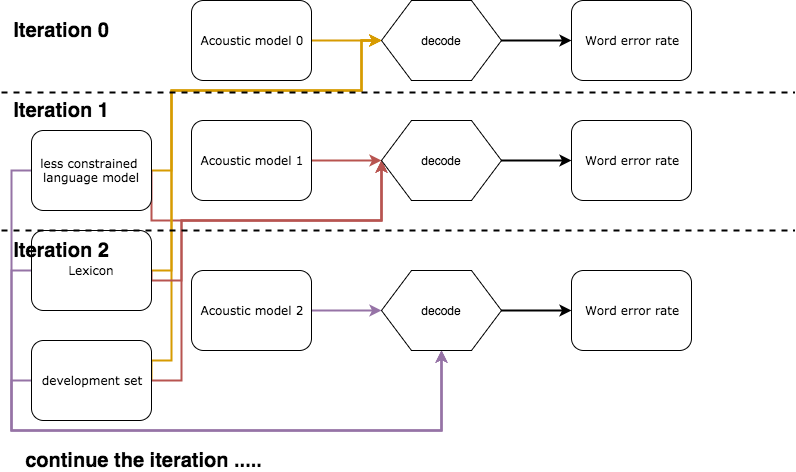
\includegraphics[scale=0.65]{EvaluationPipeline} 
\centering
\end{figure}


\begin{figure}[H]
\caption{Data selection pipeline}
\label{selectionPipeline}
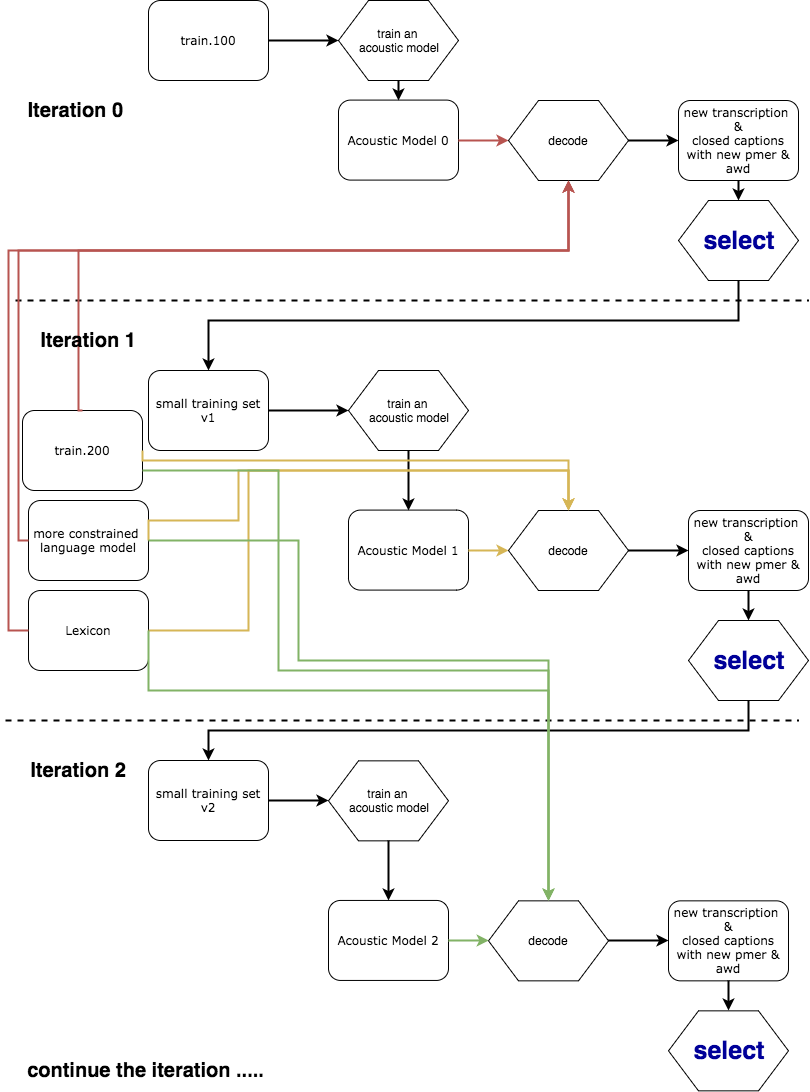
\includegraphics[scale=0.5]{DataSelection} 
\centering
\end{figure}


\subsection{Building the speech recognition systems}
The previous section explains the data selection process. Nevertheless, it does not elaborate the way to train the acoustic model and decode. This section elaborates how the speech recognizer works together as illustrated in the figure \ref{ASRchart}.

Before training an acoustic model, it is necessary to turn the audio data into a sequence of acoustic feature. The audio will be divided into small chunks and each chunk will be converted into a feature vector. 

The hybrid HMM acoustic model is the approach to build the language model as explained in the section \ref{HybridAcousticModel}. Training TDNN needs a training dataset which has training labels. Nevertheless, the training dataset only has several utterances with start and end time. It is our job to label each acoustic feature input(each small chunk of acoustic audio) with their corresponding senone. GMM-HMM is able to be trained  on  the flat start. The closed captions and the audio data are  the inputs of GMM acoustic model training. After training GMM, GMM forces alignment of each audio chunk and label them with their senone. Closed captions might not be perfect for GMM force alignment since they are not exactly the same as the real transcription.  The word error rate may be poor in the first iteration; thus we need to do data selection in the next iteration. 

After force aligning and labelling the acoustic inputs, TDNN acoustic model is trained. The TDNN acoustic model, the less constrained language model, and the lexicon are combined together to make a decoding graph. The decoding graph is based on weighted finite state transducer(WFST). WFST is a finite automata whose state transition is labeled with input, output, and a weight which encodes a probability to go to the next state. The transition maps the input symbol sequence to an output string. WFST is able to encode HMM, lexicon, and n-gram language model \cite{Mohri2008}. Thus, WFST is a perfect representation which maps the acoustic input to a word string. 

When decoding an audio dataset, the decoder does not return the most probable sentence given the acoustic inputs. Instead, it returns a directed graph containing the subset of possible paths to generate a probable sentence. This directed graph is called lattice. The nodes in lattice represent points in time, while the transitions represent states of combination acoustic model, language model, and lexicon. The lattice can be used later for decoding and rescoring with different language model or acoustic model \cite{Murveit1993}. From the generated lattice, we can search the best sequence with different and more sophisticated(but slower to do) configuration or more complex language model.


\begin{figure}[H]
\caption{Training and decoding with the speech recognition system}
\label{ASRchart}
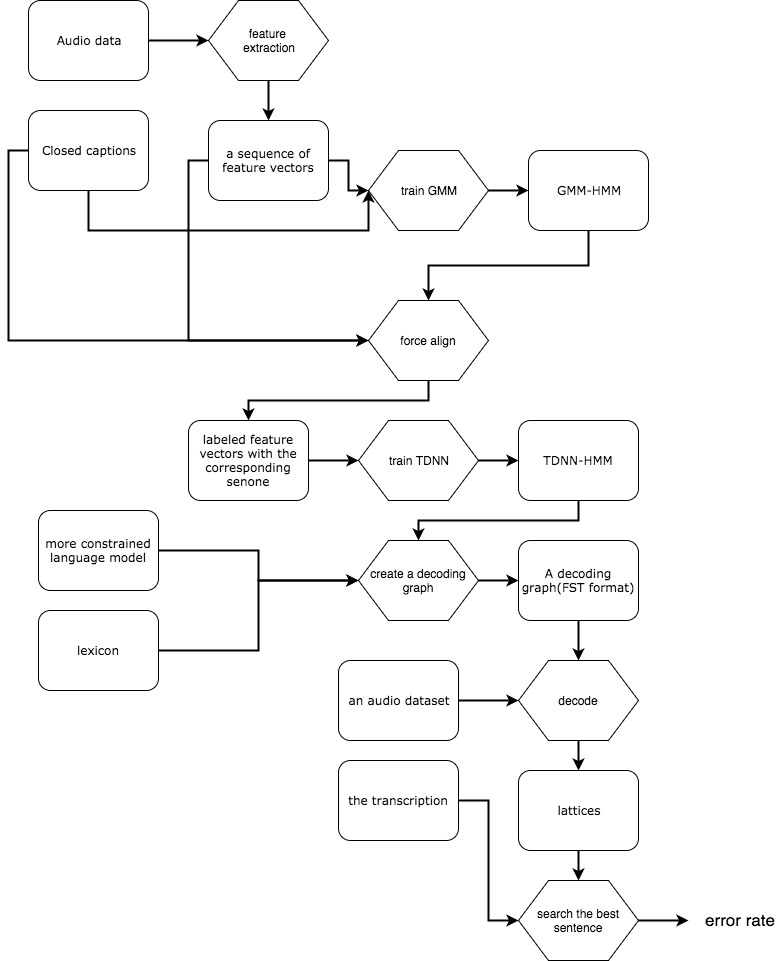
\includegraphics[scale=0.5]{TrainingAM} 
\centering
\end{figure}

\section{New proposed models}
\label{proposedModels}
The general idea of the proposed models is to combine three different automatic speech recognition(ASR) systems by varying the language model but the same acoustic model. Combining three different ASRs is expected to complement and fix other ASR's mistake. 

The language models are built with different constraints(the least, medium, and the most constraint language models). The proposed models work almost the same as the baseline model: training acoustic model with the subset of training data(audio data and their closed captions), recognizing and selecting the full training data, and repeating the steps to do more data selection. However, the difference is when recognizing and selecting data. Three different ASRs recognize the full training set, combine, and select the decoding results as following:
\begin{enumerate}
\item Average PMER and AWD of three ASRs. \\
Three different ASRs recognize the full training set and compute new values of PMER and AWD. Each corresponding segment in three ASRs averages their PMER and AWD. The average PMER and AWD are utilized to do the data selection(the same data selection as explained in the baseline model).

\item Combine PMER and AWD of three ASRs with a proposed combination algorithm \\
Here is the pseudocode how the algorithm works.
\begin{lstlisting}[caption={the proposed combination algorithm}, label={algoCombine}]
For each segment:
    Keep only segments which are in 0.166<AWD<0.65 
    and 0.03<APD(Average phone duration)<0.25 range
        If one ASR segment has zero PMER, 
            Select the segment and corresponding closed 
            captions
        Else 
            If two segments have the same phone sequence 
                Select the segment and the corresponding 
                decoding result transcription 
            Else 
                Sort by PMER. Choose top segments with 
                the lowest PMER. The closed captions will 
                be chosen.
\end{lstlisting}
There are some intuitions behind the pseudocode:
\begin{itemize}
\item Average phone duration(APD) is introduced to detect whether the segments are properly recognized by the speech recognizer in phone level. In contrast, AWD  The duration of a phone must be between 0.03 second and 0.25 second.

\begin{equation}
APD = \frac{\#\textrm{phones in the segments}}{\textrm{duration of the segment}}
\end{equation}

\item Line 8-10 is expected to fix the closed captions with the correct transcription. The closed captions are not exactly the same as the real transcriptions. When two different ASRs yield exactly the same decoding transcription, the decoding transcriptions probably matches closer to the real transcription compared to the corresponding closed captions.

\end{itemize}

\item Utilize a randomly different training set for each iteration. \\
In our baseline model, we always recognize the same full training set and select the best subset from the training set. Instead of using the same training set, we randomly choose a new full training set with more or less the same total speech duration. The intuition behind this is randomness may increase the performance of the model.

\end{enumerate}

